\documentclass[twoside]{book}

% Packages required by doxygen
\usepackage{fixltx2e}
\usepackage{calc}
\usepackage{doxygen}
\usepackage[export]{adjustbox} % also loads graphicx
\usepackage{graphicx}
\usepackage[utf8]{inputenc}
\usepackage{makeidx}
\usepackage{multicol}
\usepackage{multirow}
\PassOptionsToPackage{warn}{textcomp}
\usepackage{textcomp}
\usepackage[nointegrals]{wasysym}
\usepackage[table]{xcolor}

% Font selection
\usepackage[T1]{fontenc}
\usepackage[scaled=.90]{helvet}
\usepackage{courier}
\usepackage{amssymb}
\usepackage{sectsty}
\renewcommand{\familydefault}{\sfdefault}
\allsectionsfont{%
  \fontseries{bc}\selectfont%
  \color{darkgray}%
}
\renewcommand{\DoxyLabelFont}{%
  \fontseries{bc}\selectfont%
  \color{darkgray}%
}
\newcommand{\+}{\discretionary{\mbox{\scriptsize$\hookleftarrow$}}{}{}}

% Page & text layout
\usepackage{geometry}
\geometry{%
  a4paper,%
  top=2.5cm,%
  bottom=2.5cm,%
  left=2.5cm,%
  right=2.5cm%
}
\tolerance=750
\hfuzz=15pt
\hbadness=750
\setlength{\emergencystretch}{15pt}
\setlength{\parindent}{0cm}
\setlength{\parskip}{3ex plus 2ex minus 2ex}
\makeatletter
\renewcommand{\paragraph}{%
  \@startsection{paragraph}{4}{0ex}{-1.0ex}{1.0ex}{%
    \normalfont\normalsize\bfseries\SS@parafont%
  }%
}
\renewcommand{\subparagraph}{%
  \@startsection{subparagraph}{5}{0ex}{-1.0ex}{1.0ex}{%
    \normalfont\normalsize\bfseries\SS@subparafont%
  }%
}
\makeatother

% Headers & footers
\usepackage{fancyhdr}
\pagestyle{fancyplain}
\fancyhead[LE]{\fancyplain{}{\bfseries\thepage}}
\fancyhead[CE]{\fancyplain{}{}}
\fancyhead[RE]{\fancyplain{}{\bfseries\leftmark}}
\fancyhead[LO]{\fancyplain{}{\bfseries\rightmark}}
\fancyhead[CO]{\fancyplain{}{}}
\fancyhead[RO]{\fancyplain{}{\bfseries\thepage}}
\fancyfoot[LE]{\fancyplain{}{}}
\fancyfoot[CE]{\fancyplain{}{}}
\fancyfoot[RE]{\fancyplain{}{\bfseries\scriptsize Generated by Doxygen }}
\fancyfoot[LO]{\fancyplain{}{\bfseries\scriptsize Generated by Doxygen }}
\fancyfoot[CO]{\fancyplain{}{}}
\fancyfoot[RO]{\fancyplain{}{}}
\renewcommand{\footrulewidth}{0.4pt}
\renewcommand{\chaptermark}[1]{%
  \markboth{#1}{}%
}
\renewcommand{\sectionmark}[1]{%
  \markright{\thesection\ #1}%
}

% Indices & bibliography
\usepackage{natbib}
\usepackage[titles]{tocloft}
\setcounter{tocdepth}{3}
\setcounter{secnumdepth}{5}
\makeindex

% Hyperlinks (required, but should be loaded last)
\usepackage{ifpdf}
\ifpdf
  \usepackage[pdftex,pagebackref=true]{hyperref}
\else
  \usepackage[ps2pdf,pagebackref=true]{hyperref}
\fi
\hypersetup{%
  colorlinks=true,%
  linkcolor=blue,%
  citecolor=blue,%
  unicode%
}

% Custom commands
\newcommand{\clearemptydoublepage}{%
  \newpage{\pagestyle{empty}\cleardoublepage}%
}

\usepackage{caption}
\captionsetup{labelsep=space,justification=centering,font={bf},singlelinecheck=off,skip=4pt,position=top}

%===== C O N T E N T S =====

\begin{document}

% Titlepage & ToC
\hypersetup{pageanchor=false,
             bookmarksnumbered=true,
             pdfencoding=unicode
            }
\pagenumbering{alph}
\begin{titlepage}
\vspace*{7cm}
\begin{center}%
{\Large My Project }\\
\vspace*{1cm}
{\large Generated by Doxygen 1.8.13}\\
\end{center}
\end{titlepage}
\clearemptydoublepage
\pagenumbering{roman}
\tableofcontents
\clearemptydoublepage
\pagenumbering{arabic}
\hypersetup{pageanchor=true}

%--- Begin generated contents ---
\chapter{Data Structure Index}
\section{Data Structures}
Here are the data structures with brief descriptions\+:\begin{DoxyCompactList}
\item\contentsline{section}{\hyperlink{structentity}{entity} }{\pageref{structentity}}{}
\item\contentsline{section}{\hyperlink{structquiz}{quiz} }{\pageref{structquiz}}{}
\item\contentsline{section}{\hyperlink{structrest}{rest} }{\pageref{structrest}}{}
\end{DoxyCompactList}

\chapter{File Index}
\section{File List}
Here is a list of all files with brief descriptions\+:\begin{DoxyCompactList}
\item\contentsline{section}{\hyperlink{create_8c}{create.\+c} \\*Dans ce fichier deux fichiers binaires fait les appelles }{\pageref{create_8c}}{}
\item\contentsline{section}{\hyperlink{main_8c}{main.\+c} \\*Circuit enigme quiz }{\pageref{main_8c}}{}
\item\contentsline{section}{\hyperlink{quiz_8c}{quiz.\+c} \\*Il y a ici tous les fonctions de l\textquotesingle{}enigme quiz }{\pageref{quiz_8c}}{}
\item\contentsline{section}{\hyperlink{quiz_8h}{quiz.\+h} \\*Il y a ici les structures et la liaison des procedures de l\textquotesingle{}enigme }{\pageref{quiz_8h}}{}
\end{DoxyCompactList}

\chapter{Data Structure Documentation}
\hypertarget{structprotocol}{}\section{protocol Struct Reference}
\label{structprotocol}\index{protocol@{protocol}}


{\ttfamily \#include $<$circuit.\+h$>$}

\subsection*{Data Fields}
\begin{DoxyCompactItemize}
\item 
S\+D\+L\+\_\+\+Surface $\ast$ \hyperlink{structprotocol_a83d0768fd8d86396078d1b0b28b3d56c}{image}
\item 
S\+D\+L\+\_\+\+Rect \hyperlink{structprotocol_ad65a80eae3e7e0769fc6483fc31f5f88}{pos}
\item 
int \hyperlink{structprotocol_aa90a08ca51e428e67134a86fd03c7acd}{direction}
\end{DoxyCompactItemize}


\subsection{Field Documentation}
\mbox{\Hypertarget{structprotocol_aa90a08ca51e428e67134a86fd03c7acd}\label{structprotocol_aa90a08ca51e428e67134a86fd03c7acd}} 
\index{protocol@{protocol}!direction@{direction}}
\index{direction@{direction}!protocol@{protocol}}
\subsubsection{\texorpdfstring{direction}{direction}}
{\footnotesize\ttfamily int protocol\+::direction}

\mbox{\Hypertarget{structprotocol_a83d0768fd8d86396078d1b0b28b3d56c}\label{structprotocol_a83d0768fd8d86396078d1b0b28b3d56c}} 
\index{protocol@{protocol}!image@{image}}
\index{image@{image}!protocol@{protocol}}
\subsubsection{\texorpdfstring{image}{image}}
{\footnotesize\ttfamily S\+D\+L\+\_\+\+Surface $\ast$ protocol\+::image}

\mbox{\Hypertarget{structprotocol_ad65a80eae3e7e0769fc6483fc31f5f88}\label{structprotocol_ad65a80eae3e7e0769fc6483fc31f5f88}} 
\index{protocol@{protocol}!pos@{pos}}
\index{pos@{pos}!protocol@{protocol}}
\subsubsection{\texorpdfstring{pos}{pos}}
{\footnotesize\ttfamily S\+D\+L\+\_\+\+Rect protocol\+::pos}



The documentation for this struct was generated from the following files\+:\begin{DoxyCompactItemize}
\item 
\hyperlink{circuit_8h}{circuit.\+h}\item 
\hyperlink{hack_8c}{hack.\+c}\end{DoxyCompactItemize}

\hypertarget{structsimple}{}\section{simple Struct Reference}
\label{structsimple}\index{simple@{simple}}


{\ttfamily \#include $<$circuit.\+h$>$}

\subsection*{Data Fields}
\begin{DoxyCompactItemize}
\item 
S\+D\+L\+\_\+\+Surface $\ast$ \hyperlink{structsimple_aa13dac670d4759e6fd7de7c3d2d10440}{image}
\item 
S\+D\+L\+\_\+\+Rect \hyperlink{structsimple_a87dc9ff3f1d816ced376e752e3c4c88b}{pos}
\end{DoxyCompactItemize}


\subsection{Field Documentation}
\mbox{\Hypertarget{structsimple_aa13dac670d4759e6fd7de7c3d2d10440}\label{structsimple_aa13dac670d4759e6fd7de7c3d2d10440}} 
\index{simple@{simple}!image@{image}}
\index{image@{image}!simple@{simple}}
\subsubsection{\texorpdfstring{image}{image}}
{\footnotesize\ttfamily S\+D\+L\+\_\+\+Surface $\ast$ simple\+::image}

\mbox{\Hypertarget{structsimple_a87dc9ff3f1d816ced376e752e3c4c88b}\label{structsimple_a87dc9ff3f1d816ced376e752e3c4c88b}} 
\index{simple@{simple}!pos@{pos}}
\index{pos@{pos}!simple@{simple}}
\subsubsection{\texorpdfstring{pos}{pos}}
{\footnotesize\ttfamily S\+D\+L\+\_\+\+Rect simple\+::pos}



The documentation for this struct was generated from the following files\+:\begin{DoxyCompactItemize}
\item 
\hyperlink{circuit_8h}{circuit.\+h}\item 
\hyperlink{hack_8c}{hack.\+c}\end{DoxyCompactItemize}

\chapter{File Documentation}
\hypertarget{circuit_8c}{}\section{circuit.\+c File Reference}
\label{circuit_8c}\index{circuit.\+c@{circuit.\+c}}


il y a ici tous les fonctions de l\textquotesingle{}enigme.  


{\ttfamily \#include $<$stdio.\+h$>$}\newline
{\ttfamily \#include $<$stdlib.\+h$>$}\newline
{\ttfamily \#include $<$time.\+h$>$}\newline
{\ttfamily \#include \char`\"{}/usr/include/\+S\+D\+L/\+S\+D\+L.\+h\char`\"{}}\newline
{\ttfamily \#include \char`\"{}/usr/include/\+S\+D\+L/\+S\+D\+L\+\_\+image.\+h\char`\"{}}\newline
{\ttfamily \#include \char`\"{}/usr/include/\+S\+D\+L/\+S\+D\+L\+\_\+mixer.\+h\char`\"{}}\newline
{\ttfamily \#include \char`\"{}circuit.\+h\char`\"{}}\newline
Include dependency graph for circuit.\+c\+:
\nopagebreak
\begin{figure}[H]
\begin{center}
\leavevmode
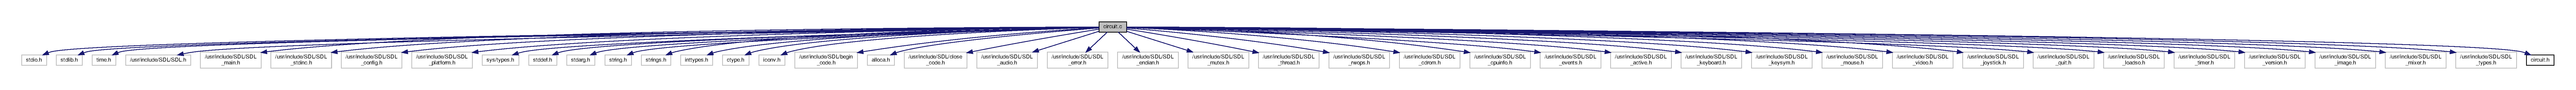
\includegraphics[width=350pt]{circuit_8c__incl}
\end{center}
\end{figure}
\subsection*{Functions}
\begin{DoxyCompactItemize}
\item 
int \hyperlink{circuit_8c_a8f387384696c4294f1521ad662b556db}{hover} (S\+D\+L\+\_\+\+Rect pos, int x, int y)
\item 
void \hyperlink{circuit_8c_a684ec0dae6d6c3e605a0fb811869ded8}{initialiser} (\hyperlink{structsimple}{simple} $\ast$screen, \hyperlink{structprotocol}{protocol} base3\mbox{[}$\,$\mbox{]}, \hyperlink{structprotocol}{protocol} base2\mbox{[}$\,$\mbox{]}, S\+D\+L\+\_\+\+Surface $\ast$pos3\mbox{[}$\,$\mbox{]}, S\+D\+L\+\_\+\+Surface $\ast$pos2\mbox{[}$\,$\mbox{]}, S\+D\+L\+\_\+\+Surface $\ast$$\ast$unlocked, S\+D\+L\+\_\+\+Surface $\ast$$\ast$lockked, \hyperlink{structsimple}{simple} $\ast$circuit, \hyperlink{structsimple}{simple} $\ast$locked, \hyperlink{structsimple}{simple} $\ast$image)
\begin{DoxyCompactList}\small\item\em initialiser les donnees de l\textquotesingle{}enigme. \end{DoxyCompactList}\item 
void \hyperlink{circuit_8c_a683586511a2c9c8b9e76a5e3fb519996}{afficher} (\hyperlink{structsimple}{simple} screen, \hyperlink{structprotocol}{protocol} base3\mbox{[}$\,$\mbox{]}, \hyperlink{structprotocol}{protocol} base2\mbox{[}$\,$\mbox{]}, S\+D\+L\+\_\+\+Surface $\ast$pos3\mbox{[}$\,$\mbox{]}, S\+D\+L\+\_\+\+Surface $\ast$pos2\mbox{[}$\,$\mbox{]}, S\+D\+L\+\_\+\+Surface $\ast$unlocked, S\+D\+L\+\_\+\+Surface $\ast$lockked, \hyperlink{structsimple}{simple} circuit, \hyperlink{structsimple}{simple} $\ast$locked, S\+D\+L\+\_\+\+Event event, \hyperlink{structsimple}{simple} image)
\begin{DoxyCompactList}\small\item\em afficher et modifier les donnees de l\textquotesingle{}enigme. \end{DoxyCompactList}\end{DoxyCompactItemize}


\subsection{Detailed Description}
il y a ici tous les fonctions de l\textquotesingle{}enigme. 



\subsection{Function Documentation}
\mbox{\Hypertarget{circuit_8c_a683586511a2c9c8b9e76a5e3fb519996}\label{circuit_8c_a683586511a2c9c8b9e76a5e3fb519996}} 
\index{circuit.\+c@{circuit.\+c}!afficher@{afficher}}
\index{afficher@{afficher}!circuit.\+c@{circuit.\+c}}
\subsubsection{\texorpdfstring{afficher()}{afficher()}}
{\footnotesize\ttfamily void afficher (\begin{DoxyParamCaption}\item[{\hyperlink{structsimple}{simple}}]{screen,  }\item[{\hyperlink{structprotocol}{protocol}}]{base3\mbox{[}$\,$\mbox{]},  }\item[{\hyperlink{structprotocol}{protocol}}]{base2\mbox{[}$\,$\mbox{]},  }\item[{S\+D\+L\+\_\+\+Surface $\ast$}]{pos3\mbox{[}$\,$\mbox{]},  }\item[{S\+D\+L\+\_\+\+Surface $\ast$}]{pos2\mbox{[}$\,$\mbox{]},  }\item[{S\+D\+L\+\_\+\+Surface $\ast$}]{unlocked,  }\item[{S\+D\+L\+\_\+\+Surface $\ast$}]{lockked,  }\item[{\hyperlink{structsimple}{simple}}]{circuit,  }\item[{\hyperlink{structsimple}{simple} $\ast$}]{locked,  }\item[{S\+D\+L\+\_\+\+Event}]{event,  }\item[{\hyperlink{structsimple}{simple}}]{image }\end{DoxyParamCaption})}



afficher et modifier les donnees de l\textquotesingle{}enigme. 


\begin{DoxyParams}{Parameters}
{\em simple} & screen \+: affiche l\textquotesingle{}ecran. \\
\hline
{\em protocol} & base3\mbox{[}\mbox{]},base2\mbox{[}\mbox{]} \+: change surface des liaisons electriques. \\
\hline
{\em S\+D\+L\+\_\+\+Surface} & pos3\mbox{[}\mbox{]},pos2\mbox{[}\mbox{]}\+: les differents liaisons qu\textquotesingle{}il faut prendre et changer dans le circuit. \\
\hline
{\em S\+D\+L\+\_\+\+Event} & event \+: fait les actions generer pas le hardware. \\
\hline
{\em simple} & circuit \+: affiche la base circuit avec sa position. \\
\hline
\end{DoxyParams}
\begin{DoxyReturn}{Returns}
affichage de l\textquotesingle{}enigme. 
\end{DoxyReturn}
Here is the call graph for this function\+:\nopagebreak
\begin{figure}[H]
\begin{center}
\leavevmode
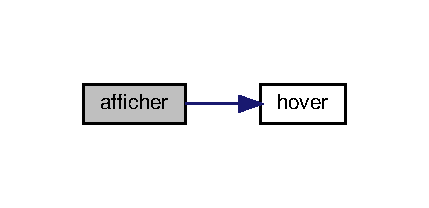
\includegraphics[width=206pt]{circuit_8c_a683586511a2c9c8b9e76a5e3fb519996_cgraph}
\end{center}
\end{figure}
Here is the caller graph for this function\+:\nopagebreak
\begin{figure}[H]
\begin{center}
\leavevmode
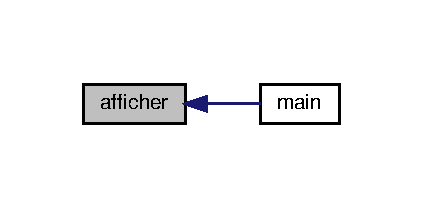
\includegraphics[width=203pt]{circuit_8c_a683586511a2c9c8b9e76a5e3fb519996_icgraph}
\end{center}
\end{figure}
\mbox{\Hypertarget{circuit_8c_a8f387384696c4294f1521ad662b556db}\label{circuit_8c_a8f387384696c4294f1521ad662b556db}} 
\index{circuit.\+c@{circuit.\+c}!hover@{hover}}
\index{hover@{hover}!circuit.\+c@{circuit.\+c}}
\subsubsection{\texorpdfstring{hover()}{hover()}}
{\footnotesize\ttfamily int hover (\begin{DoxyParamCaption}\item[{S\+D\+L\+\_\+\+Rect}]{pos,  }\item[{int}]{x,  }\item[{int}]{y }\end{DoxyParamCaption})}

Here is the caller graph for this function\+:\nopagebreak
\begin{figure}[H]
\begin{center}
\leavevmode
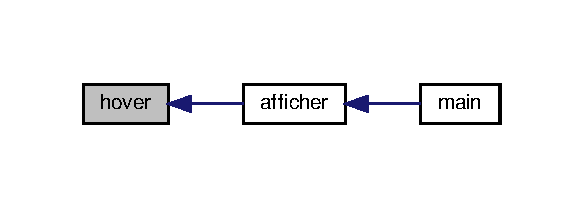
\includegraphics[width=280pt]{circuit_8c_a8f387384696c4294f1521ad662b556db_icgraph}
\end{center}
\end{figure}
\mbox{\Hypertarget{circuit_8c_a684ec0dae6d6c3e605a0fb811869ded8}\label{circuit_8c_a684ec0dae6d6c3e605a0fb811869ded8}} 
\index{circuit.\+c@{circuit.\+c}!initialiser@{initialiser}}
\index{initialiser@{initialiser}!circuit.\+c@{circuit.\+c}}
\subsubsection{\texorpdfstring{initialiser()}{initialiser()}}
{\footnotesize\ttfamily void initialiser (\begin{DoxyParamCaption}\item[{\hyperlink{structsimple}{simple} $\ast$}]{screen,  }\item[{\hyperlink{structprotocol}{protocol}}]{base3\mbox{[}$\,$\mbox{]},  }\item[{\hyperlink{structprotocol}{protocol}}]{base2\mbox{[}$\,$\mbox{]},  }\item[{S\+D\+L\+\_\+\+Surface $\ast$}]{pos3\mbox{[}$\,$\mbox{]},  }\item[{S\+D\+L\+\_\+\+Surface $\ast$}]{pos2\mbox{[}$\,$\mbox{]},  }\item[{S\+D\+L\+\_\+\+Surface $\ast$$\ast$}]{unlocked,  }\item[{S\+D\+L\+\_\+\+Surface $\ast$$\ast$}]{lockked,  }\item[{\hyperlink{structsimple}{simple} $\ast$}]{circuit,  }\item[{\hyperlink{structsimple}{simple} $\ast$}]{locked,  }\item[{\hyperlink{structsimple}{simple} $\ast$}]{image }\end{DoxyParamCaption})}



initialiser les donnees de l\textquotesingle{}enigme. 


\begin{DoxyParams}{Parameters}
{\em simple} & $\ast$screen,$\ast$locked,$\ast$image \+: adresse pour changer avec surface et position de l\textquotesingle{}ecran,disponibilité et le background. \\
\hline
{\em protocol} & base3\mbox{[}\mbox{]},base2\mbox{[}\mbox{]} \+: different protocols pour liaison du circuit avec position et surface. \\
\hline
{\em S\+D\+L\+\_\+\+Surface$\ast$} & pos3\mbox{[}\mbox{]},pos2\mbox{[}\mbox{]} \+: images des differents positions du protocol. \\
\hline
\end{DoxyParams}
\begin{DoxyReturn}{Returns}
Initialisation de l\textquotesingle{}enigme 
\end{DoxyReturn}
Here is the caller graph for this function\+:\nopagebreak
\begin{figure}[H]
\begin{center}
\leavevmode
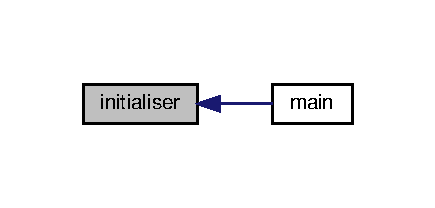
\includegraphics[width=209pt]{circuit_8c_a684ec0dae6d6c3e605a0fb811869ded8_icgraph}
\end{center}
\end{figure}

\hypertarget{circuit_8h}{}\section{circuit.\+h File Reference}
\label{circuit_8h}\index{circuit.\+h@{circuit.\+h}}


il y a ici les structures et la liaison des procedures de l\textquotesingle{}enigme.  


This graph shows which files directly or indirectly include this file\+:\nopagebreak
\begin{figure}[H]
\begin{center}
\leavevmode
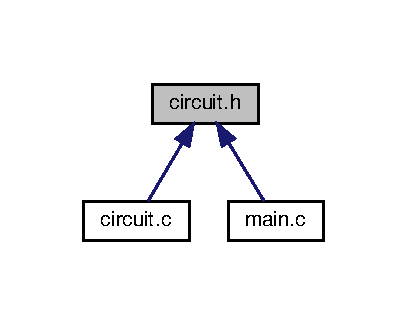
\includegraphics[width=196pt]{circuit_8h__dep__incl}
\end{center}
\end{figure}
\subsection*{Data Structures}
\begin{DoxyCompactItemize}
\item 
struct \hyperlink{structprotocol}{protocol}
\item 
struct \hyperlink{structsimple}{simple}
\end{DoxyCompactItemize}
\subsection*{Functions}
\begin{DoxyCompactItemize}
\item 
int \hyperlink{circuit_8h_a8f387384696c4294f1521ad662b556db}{hover} (S\+D\+L\+\_\+\+Rect pos, int x, int y)
\item 
void \hyperlink{circuit_8h_a684ec0dae6d6c3e605a0fb811869ded8}{initialiser} (\hyperlink{structsimple}{simple} $\ast$screen, \hyperlink{structprotocol}{protocol} base3\mbox{[}$\,$\mbox{]}, \hyperlink{structprotocol}{protocol} base2\mbox{[}$\,$\mbox{]}, S\+D\+L\+\_\+\+Surface $\ast$pos3\mbox{[}$\,$\mbox{]}, S\+D\+L\+\_\+\+Surface $\ast$pos2\mbox{[}$\,$\mbox{]}, S\+D\+L\+\_\+\+Surface $\ast$$\ast$unlocked, S\+D\+L\+\_\+\+Surface $\ast$$\ast$lockked, \hyperlink{structsimple}{simple} $\ast$circuit, \hyperlink{structsimple}{simple} $\ast$locked, \hyperlink{structsimple}{simple} $\ast$image)
\begin{DoxyCompactList}\small\item\em initialiser les donnees de l\textquotesingle{}enigme. \end{DoxyCompactList}\item 
void \hyperlink{circuit_8h_a683586511a2c9c8b9e76a5e3fb519996}{afficher} (\hyperlink{structsimple}{simple} screen, \hyperlink{structprotocol}{protocol} base3\mbox{[}$\,$\mbox{]}, \hyperlink{structprotocol}{protocol} base2\mbox{[}$\,$\mbox{]}, S\+D\+L\+\_\+\+Surface $\ast$pos3\mbox{[}$\,$\mbox{]}, S\+D\+L\+\_\+\+Surface $\ast$pos2\mbox{[}$\,$\mbox{]}, S\+D\+L\+\_\+\+Surface $\ast$unlocked, S\+D\+L\+\_\+\+Surface $\ast$lockked, \hyperlink{structsimple}{simple} circuit, \hyperlink{structsimple}{simple} $\ast$locked, S\+D\+L\+\_\+\+Event event, \hyperlink{structsimple}{simple} image)
\begin{DoxyCompactList}\small\item\em afficher et modifier les donnees de l\textquotesingle{}enigme. \end{DoxyCompactList}\end{DoxyCompactItemize}


\subsection{Detailed Description}
il y a ici les structures et la liaison des procedures de l\textquotesingle{}enigme. 



\subsection{Function Documentation}
\mbox{\Hypertarget{circuit_8h_a683586511a2c9c8b9e76a5e3fb519996}\label{circuit_8h_a683586511a2c9c8b9e76a5e3fb519996}} 
\index{circuit.\+h@{circuit.\+h}!afficher@{afficher}}
\index{afficher@{afficher}!circuit.\+h@{circuit.\+h}}
\subsubsection{\texorpdfstring{afficher()}{afficher()}}
{\footnotesize\ttfamily void afficher (\begin{DoxyParamCaption}\item[{\hyperlink{structsimple}{simple}}]{screen,  }\item[{\hyperlink{structprotocol}{protocol}}]{base3\mbox{[}$\,$\mbox{]},  }\item[{\hyperlink{structprotocol}{protocol}}]{base2\mbox{[}$\,$\mbox{]},  }\item[{S\+D\+L\+\_\+\+Surface $\ast$}]{pos3\mbox{[}$\,$\mbox{]},  }\item[{S\+D\+L\+\_\+\+Surface $\ast$}]{pos2\mbox{[}$\,$\mbox{]},  }\item[{S\+D\+L\+\_\+\+Surface $\ast$}]{unlocked,  }\item[{S\+D\+L\+\_\+\+Surface $\ast$}]{lockked,  }\item[{\hyperlink{structsimple}{simple}}]{circuit,  }\item[{\hyperlink{structsimple}{simple} $\ast$}]{locked,  }\item[{S\+D\+L\+\_\+\+Event}]{event,  }\item[{\hyperlink{structsimple}{simple}}]{image }\end{DoxyParamCaption})}



afficher et modifier les donnees de l\textquotesingle{}enigme. 


\begin{DoxyParams}{Parameters}
{\em simple} & screen \+: affiche l\textquotesingle{}ecran. \\
\hline
{\em protocol} & base3\mbox{[}\mbox{]},base2\mbox{[}\mbox{]} \+: change surface des liaisons electriques. \\
\hline
{\em S\+D\+L\+\_\+\+Surface} & pos3\mbox{[}\mbox{]},pos2\mbox{[}\mbox{]}\+: les differents liaisons qu\textquotesingle{}il faut prendre et changer dans le circuit. \\
\hline
{\em S\+D\+L\+\_\+\+Event} & event \+: fait les actions generer pas le hardware. \\
\hline
{\em simple} & circuit \+: affiche la base circuit avec sa position. \\
\hline
\end{DoxyParams}
\begin{DoxyReturn}{Returns}
affichage de l\textquotesingle{}enigme. 
\end{DoxyReturn}
Here is the call graph for this function\+:\nopagebreak
\begin{figure}[H]
\begin{center}
\leavevmode
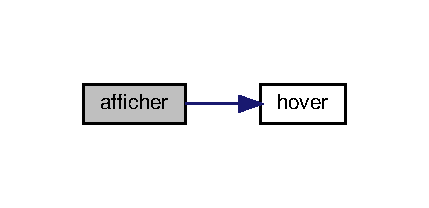
\includegraphics[width=206pt]{circuit_8h_a683586511a2c9c8b9e76a5e3fb519996_cgraph}
\end{center}
\end{figure}
Here is the caller graph for this function\+:\nopagebreak
\begin{figure}[H]
\begin{center}
\leavevmode
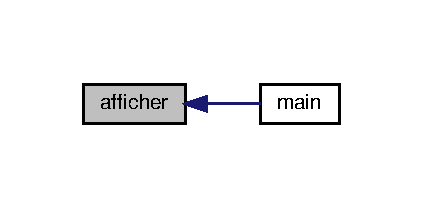
\includegraphics[width=203pt]{circuit_8h_a683586511a2c9c8b9e76a5e3fb519996_icgraph}
\end{center}
\end{figure}
\mbox{\Hypertarget{circuit_8h_a8f387384696c4294f1521ad662b556db}\label{circuit_8h_a8f387384696c4294f1521ad662b556db}} 
\index{circuit.\+h@{circuit.\+h}!hover@{hover}}
\index{hover@{hover}!circuit.\+h@{circuit.\+h}}
\subsubsection{\texorpdfstring{hover()}{hover()}}
{\footnotesize\ttfamily int hover (\begin{DoxyParamCaption}\item[{S\+D\+L\+\_\+\+Rect}]{pos,  }\item[{int}]{x,  }\item[{int}]{y }\end{DoxyParamCaption})}

Here is the caller graph for this function\+:\nopagebreak
\begin{figure}[H]
\begin{center}
\leavevmode
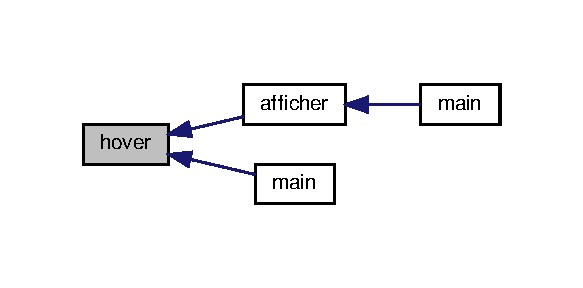
\includegraphics[width=280pt]{circuit_8h_a8f387384696c4294f1521ad662b556db_icgraph}
\end{center}
\end{figure}
\mbox{\Hypertarget{circuit_8h_a684ec0dae6d6c3e605a0fb811869ded8}\label{circuit_8h_a684ec0dae6d6c3e605a0fb811869ded8}} 
\index{circuit.\+h@{circuit.\+h}!initialiser@{initialiser}}
\index{initialiser@{initialiser}!circuit.\+h@{circuit.\+h}}
\subsubsection{\texorpdfstring{initialiser()}{initialiser()}}
{\footnotesize\ttfamily void initialiser (\begin{DoxyParamCaption}\item[{\hyperlink{structsimple}{simple} $\ast$}]{screen,  }\item[{\hyperlink{structprotocol}{protocol}}]{base3\mbox{[}$\,$\mbox{]},  }\item[{\hyperlink{structprotocol}{protocol}}]{base2\mbox{[}$\,$\mbox{]},  }\item[{S\+D\+L\+\_\+\+Surface $\ast$}]{pos3\mbox{[}$\,$\mbox{]},  }\item[{S\+D\+L\+\_\+\+Surface $\ast$}]{pos2\mbox{[}$\,$\mbox{]},  }\item[{S\+D\+L\+\_\+\+Surface $\ast$$\ast$}]{unlocked,  }\item[{S\+D\+L\+\_\+\+Surface $\ast$$\ast$}]{lockked,  }\item[{\hyperlink{structsimple}{simple} $\ast$}]{circuit,  }\item[{\hyperlink{structsimple}{simple} $\ast$}]{locked,  }\item[{\hyperlink{structsimple}{simple} $\ast$}]{image }\end{DoxyParamCaption})}



initialiser les donnees de l\textquotesingle{}enigme. 


\begin{DoxyParams}{Parameters}
{\em simple} & $\ast$screen,$\ast$locked,$\ast$image \+: adresse pour changer avec surface et position de l\textquotesingle{}ecran,disponibilité et le background. \\
\hline
{\em protocol} & base3\mbox{[}\mbox{]},base2\mbox{[}\mbox{]} \+: different protocols pour liaison du circuit avec position et surface. \\
\hline
{\em S\+D\+L\+\_\+\+Surface$\ast$} & pos3\mbox{[}\mbox{]},pos2\mbox{[}\mbox{]} \+: images des differents positions du protocol. \\
\hline
\end{DoxyParams}
\begin{DoxyReturn}{Returns}
Initialisation de l\textquotesingle{}enigme 
\end{DoxyReturn}
Here is the caller graph for this function\+:\nopagebreak
\begin{figure}[H]
\begin{center}
\leavevmode
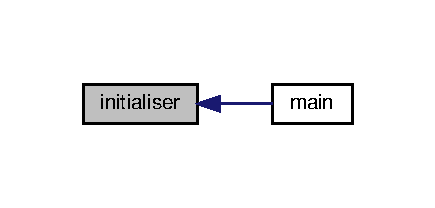
\includegraphics[width=209pt]{circuit_8h_a684ec0dae6d6c3e605a0fb811869ded8_icgraph}
\end{center}
\end{figure}

\hypertarget{hack_8c}{}\section{hack.\+c File Reference}
\label{hack_8c}\index{hack.\+c@{hack.\+c}}
{\ttfamily \#include $<$stdio.\+h$>$}\newline
{\ttfamily \#include $<$stdlib.\+h$>$}\newline
{\ttfamily \#include \char`\"{}/usr/include/\+S\+D\+L/\+S\+D\+L.\+h\char`\"{}}\newline
{\ttfamily \#include \char`\"{}/usr/include/\+S\+D\+L/\+S\+D\+L\+\_\+image.\+h\char`\"{}}\newline
{\ttfamily \#include \char`\"{}/usr/include/\+S\+D\+L/\+S\+D\+L\+\_\+mixer.\+h\char`\"{}}\newline
{\ttfamily \#include \char`\"{}/usr/include/\+S\+D\+L/\+S\+D\+L\+\_\+events.\+h\char`\"{}}\newline
{\ttfamily \#include \char`\"{}/usr/include/\+S\+D\+L/\+S\+D\+L\+\_\+mouse.\+h\char`\"{}}\newline
Include dependency graph for hack.\+c\+:\nopagebreak
\begin{figure}[H]
\begin{center}
\leavevmode
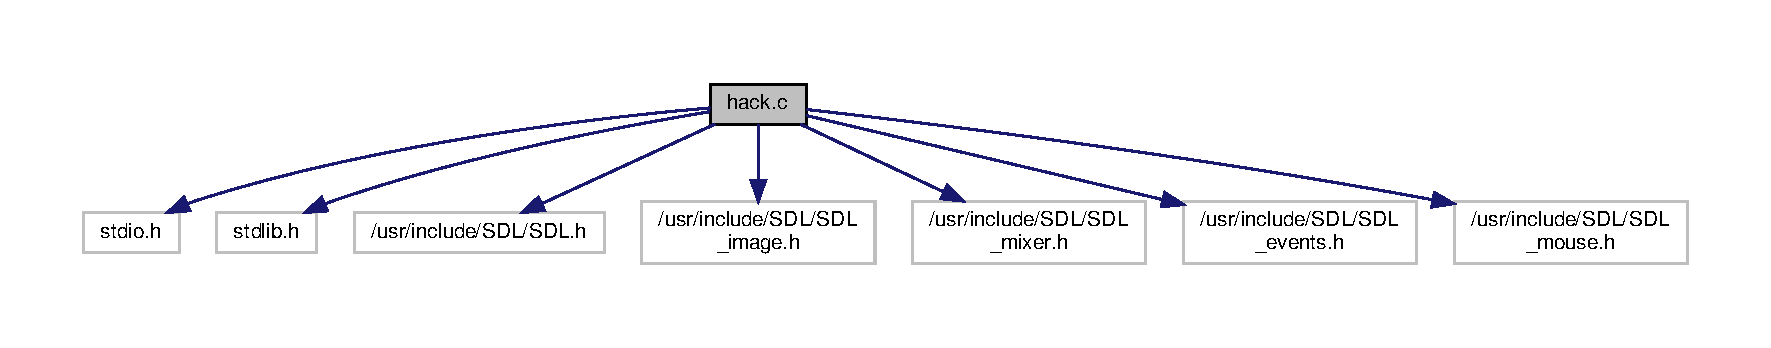
\includegraphics[width=350pt]{hack_8c__incl}
\end{center}
\end{figure}
\subsection*{Data Structures}
\begin{DoxyCompactItemize}
\item 
struct \hyperlink{structprotocol}{protocol}
\item 
struct \hyperlink{structsimple}{simple}
\end{DoxyCompactItemize}
\subsection*{Functions}
\begin{DoxyCompactItemize}
\item 
int \hyperlink{hack_8c_a8f387384696c4294f1521ad662b556db}{hover} (S\+D\+L\+\_\+\+Rect pos, int x, int y)
\item 
void \hyperlink{hack_8c_acdef7a1fd863a6d3770c1268cb06add3}{main} ()
\end{DoxyCompactItemize}


\subsection{Function Documentation}
\mbox{\Hypertarget{hack_8c_a8f387384696c4294f1521ad662b556db}\label{hack_8c_a8f387384696c4294f1521ad662b556db}} 
\index{hack.\+c@{hack.\+c}!hover@{hover}}
\index{hover@{hover}!hack.\+c@{hack.\+c}}
\subsubsection{\texorpdfstring{hover()}{hover()}}
{\footnotesize\ttfamily int hover (\begin{DoxyParamCaption}\item[{S\+D\+L\+\_\+\+Rect}]{pos,  }\item[{int}]{x,  }\item[{int}]{y }\end{DoxyParamCaption})}

Here is the caller graph for this function\+:\nopagebreak
\begin{figure}[H]
\begin{center}
\leavevmode
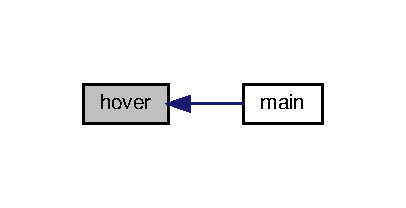
\includegraphics[width=195pt]{hack_8c_a8f387384696c4294f1521ad662b556db_icgraph}
\end{center}
\end{figure}
\mbox{\Hypertarget{hack_8c_acdef7a1fd863a6d3770c1268cb06add3}\label{hack_8c_acdef7a1fd863a6d3770c1268cb06add3}} 
\index{hack.\+c@{hack.\+c}!main@{main}}
\index{main@{main}!hack.\+c@{hack.\+c}}
\subsubsection{\texorpdfstring{main()}{main()}}
{\footnotesize\ttfamily void main (\begin{DoxyParamCaption}{ }\end{DoxyParamCaption})}

Here is the call graph for this function\+:\nopagebreak
\begin{figure}[H]
\begin{center}
\leavevmode
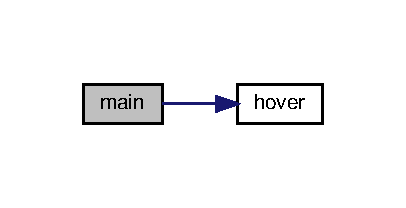
\includegraphics[width=195pt]{hack_8c_acdef7a1fd863a6d3770c1268cb06add3_cgraph}
\end{center}
\end{figure}

\hypertarget{main_8c}{}\section{main.\+c File Reference}
\label{main_8c}\index{main.\+c@{main.\+c}}


circuit enigme.  


{\ttfamily \#include $<$stdio.\+h$>$}\newline
{\ttfamily \#include $<$stdlib.\+h$>$}\newline
{\ttfamily \#include $<$time.\+h$>$}\newline
{\ttfamily \#include \char`\"{}/usr/include/\+S\+D\+L/\+S\+D\+L.\+h\char`\"{}}\newline
{\ttfamily \#include \char`\"{}/usr/include/\+S\+D\+L/\+S\+D\+L\+\_\+image.\+h\char`\"{}}\newline
{\ttfamily \#include \char`\"{}/usr/include/\+S\+D\+L/\+S\+D\+L\+\_\+mixer.\+h\char`\"{}}\newline
{\ttfamily \#include \char`\"{}/usr/include/\+S\+D\+L/\+S\+D\+L\+\_\+events.\+h\char`\"{}}\newline
{\ttfamily \#include \char`\"{}/usr/include/\+S\+D\+L/\+S\+D\+L\+\_\+mouse.\+h\char`\"{}}\newline
{\ttfamily \#include \char`\"{}circuit.\+h\char`\"{}}\newline
Include dependency graph for main.\+c\+:
\nopagebreak
\begin{figure}[H]
\begin{center}
\leavevmode
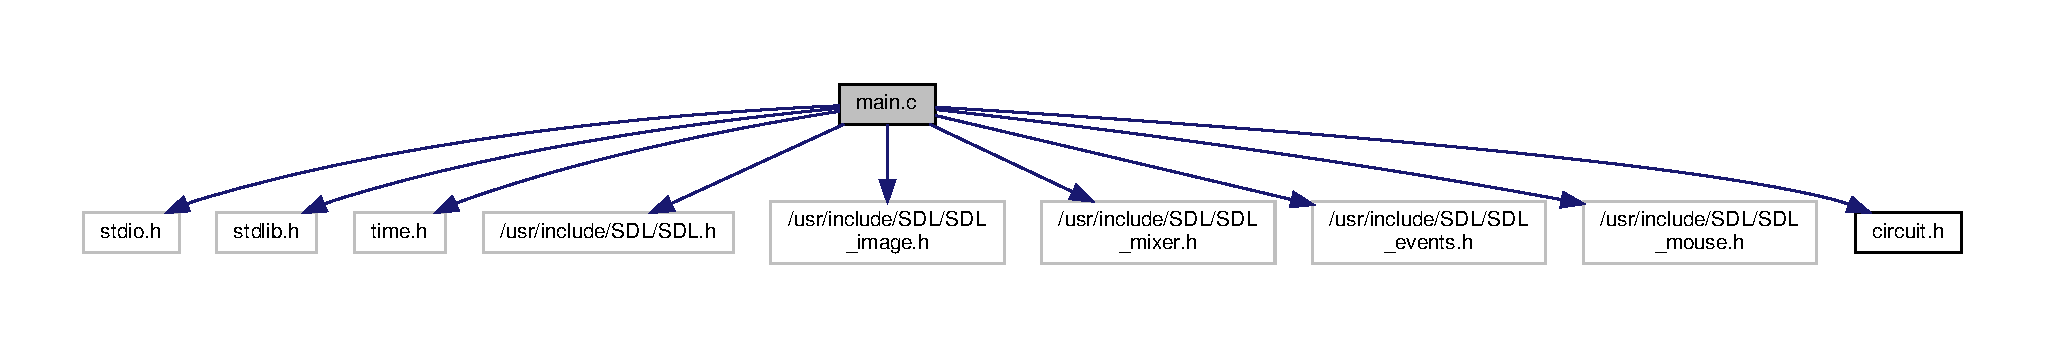
\includegraphics[width=350pt]{main_8c__incl}
\end{center}
\end{figure}
\subsection*{Functions}
\begin{DoxyCompactItemize}
\item 
int \hyperlink{main_8c_ae66f6b31b5ad750f1fe042a706a4e3d4}{main} ()
\end{DoxyCompactItemize}


\subsection{Detailed Description}
circuit enigme. 

\begin{DoxyAuthor}{Author}
Blindspot 
\end{DoxyAuthor}
\begin{DoxyVersion}{Version}
0.\+1 
\end{DoxyVersion}
\begin{DoxyDate}{Date}
M\+AY 06, 2019 
\end{DoxyDate}


\subsection{Function Documentation}
\mbox{\Hypertarget{main_8c_ae66f6b31b5ad750f1fe042a706a4e3d4}\label{main_8c_ae66f6b31b5ad750f1fe042a706a4e3d4}} 
\index{main.\+c@{main.\+c}!main@{main}}
\index{main@{main}!main.\+c@{main.\+c}}
\subsubsection{\texorpdfstring{main()}{main()}}
{\footnotesize\ttfamily int main (\begin{DoxyParamCaption}{ }\end{DoxyParamCaption})}

Here is the call graph for this function\+:\nopagebreak
\begin{figure}[H]
\begin{center}
\leavevmode
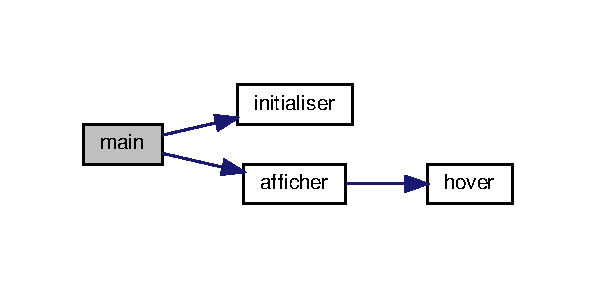
\includegraphics[width=286pt]{main_8c_ae66f6b31b5ad750f1fe042a706a4e3d4_cgraph}
\end{center}
\end{figure}

%--- End generated contents ---

% Index
\backmatter
\newpage
\phantomsection
\clearemptydoublepage
\addcontentsline{toc}{chapter}{Index}
\printindex

\end{document}
